\documentclass{article}

% Language setting
% Replace `english' with e.g. `spanish' to change the document language
\usepackage[english]{babel}

% Set page size and margins
% Replace `letterpaper' with `a4paper' for UK/EU standard size
\usepackage[letterpaper,top=2cm,bottom=2cm,left=3cm,right=3cm,marginparwidth=1.75cm]{geometry}
\usepackage{pythonhighlight}
\usepackage{color,soul}

% Useful packages
\usepackage{amsmath}
\usepackage{graphicx}
\usepackage[colorlinks=true, allcolors=blue]{hyperref}


% maximum / minimum over fixed length lists, over variable length lists, how does that change?
\title{Mechanistic Interpretability of Maximum of Variable Length Lists}
\author{Eric Wang}

\begin{document}
\maketitle

\section{Introduction}

Interpretability is a field of growing importance with the development of AI. It refers to the study of understanding how machine learning machines work and how they make decisions. This is especially important in the development of safe, reliable AI because then we are able to predict how an AI system might behave when deployed. However, there is a lack of understanding with current AI systems. Thus, in this project, I aim to preform simple interpretability on a small transformer model trained to take the maximum of variable length lists in order to gain some practice in interpretability and working with transformers.

In this paper, I aim to reverse engineer a model that is trained to take the maximum of variable length lists and some variations of this problem to perform mechanistic interpretability. Notably, I will be taking inspiration from one of the ``200 Concrete Open Problems in Mechanistic Interpretability'' as described by Neel Nanda. The goal of this project is to train the model to complete this synthetic, algorithmic task because when models are trained on these kind of simple tasks, it results in clean, interpretable computation \cite{1}. Oftentimes, the way that the model goes about solving a simple algorithmic problem is the not the same as a human would go about solving the problem. For example, instead of doing modular addition, a trained model might learn to do a trig-based algorithm instead.

By building this simple model on an algorithmic task, I hope to uncover the inner workings of the model and how it learns to take the maximum of lists. I also hope to gain experience writing a transformer from scratch and understanding how it works at a basic level. I anticipate seeing phenomenon such as Grokking, where small models trained on algorithmic tasks memorize the training data and overfit on it, but then after doing more training suddenly learn how to generalize. Ultimately, I hope to practice writing and training machine learning models and do some interpretability on the results. My end goal is to gain some experience working with transformers, and get practice with interpretability. 

\section{Literature Review}

We will first start with a brief literature review. In order to write a transformer from scratch, I heavily depended on the original transformer paper ``Attention Is All You Need'' \cite{6}. This paper introduces the transformer model and the attention mechanism. The description of the key, value, and query matrices and how they are used to calculate the attention weights among other mechanisms were key to understanding and implementing the transformer model.

I also took inspiration from ``A Multiscale Visualization of Attention in the Transformer Model" \cite{7} when working with interpreting the results of the transformer model. In this paper, they describe the complexity of deciphering multi-layer, multi-head attention mechanisms, and introduce a visualization tool to simplify the behavior. They were able to detect model bias, locate relevant attention heads, and link neurons to model behavior. This paper was key in understanding how I should go about interpreting the results of my experiment.

I am drawing heavy inspiration and modeling my project after Neel Nanda's ``A Mechanistic Interpretability Analysis of Grokking,"\cite{2} where he trains a model to do modular addition and reverse engineers how the model works. He discovers that grokking occurs at a crossover point, where the model goes from memorizing the data to generalizing data. I plan to do similar analyses and reverse engineering methods as he does to investigate the inner workings of the model I train with the goal of gaining more practice working with ML and interpretability research. I expect that I will have similar results to him, and although he has addressed the broad question, there hasn't been projects done directly addressing finding the maximum across variable length lists. Thus, I want to use this algorithmic problem to practice and reverse engineer to see if I can extend to new findings.

Throughout the project, I will also be following along tips and reverse engineering methods as described in Neel Nanda's blog post ``200 COP in MI: The Case for Analysing Toy Language Models'' \cite{3}. The algorithmic problem I'm addressing is an extension of a problem proposed in this blog post, where instead of finding the maximum of two numbers, I will experiment with finding the maximum of a number in a fixed length list and extend it to finding the maximum number of a variable length list. 

\section{Project Setup}

\subsection{Transformer from Scratch}

First, I wanted to gain practice by writing a transformer from scratch. I was able to do this by following the description of the transformer in the paper "Attention is All You Need" \cite{7}. I did this by using PyTorch and building ontop of the nn.Module class, which is a class within PyTorch that helps define neural networks. 

At the heart of transformers are the query, key, and value mechanisms. At a high level, we can view the keys as information we have that maps to some values. The query is what we want to look up against this set of keys, which are associated with values. The attention mechanism then serves as a ``compatibility function of the query and the corresponding key." that finds the most compatible key and corresponding value \cite{7}. In other words, for each given query, a probability distribution is calculated for how much care should be given to a specific key. In our case, the query, key, and value will all be generated from the input data, and this is called self-attention. 

To replicate this concept in code, I used the nn.Module class to create a SimpleTransformer class. Within this class, I defined the initialization function,
where I created layers for the embedding, query, key, value, and feed forward network. The query, key, and value mechanisms are created using the nn.Linear function because these are all learnable parameters that will be updated as the model trains. Furthermore, the feed forward network is composed of a simple linear layer followed by a ReLU activation function and another linear layer. This is to keep the model relatively simple since the tasks I am training the model on are simple algorithmic problems.

Within this transformer, I also implemented the forward function, which is the function that is called when the model is run on the input tokens. This function embeds the input data, and then calculates the query, key, and values for the attention mechanism. The attention weights are then calculated using this equation:

$$
\text{Attention}(Q, K, V) = \text{softmax}\left(\frac{QK^T}{\sqrt{d_k}}\right)V
$$

which is at the core of how the transformer model works. The output of the attention mechanism is then calculated by passing the attention weights through the feed forward network. The code for this is in the file named ``scratch$\_$transform.ipynb''.

After writing this simple transformer, I was able to train it on a simple task. Specifically, I trained the model to take the maximum of a fixed length list of numbers. The specifics of training a model to do this will be detailed in the subsequent sections.

\subsection{Transformer Lens}

Now that we have experience creating transformers from scratch and training them on simple tasks, we can move on to the main task of this project, which is interpreting the transformer model and seeing what it learned. This is hard to do so with the normal transformer model that was written from scratch because other than the weights, it is hard to visualize the attention patterns or any of the activations. Thus, I opted to use the Transformer Lens library crated by Neel Nanda \cite{9}, which attaches hooks to every important activation in the model such that attention heads can be visualized. 

The most important part of this library is defining the config for the transformer model, which includes the dimension of the model, number of layers, number of heads, context length, vocab size, and the activation function among other parameters. Once the config is defined, the transformer model should work the same as the one we wrote from scratch. The other implementations are abstracted away, so we will assume that the library works as intended and we will use this moving forward. An example of how this is implemented is shown below:

\begin{python}
cfg = HookedTransformerConfig(
    d_model=32,
    n_layers=1,
    n_heads=1,
    d_head=32,
    n_ctx=10,
    d_vocab=64,
    act_fn="relu",
    seed=123,
    device="mps",
    attn_only=True,
)

model = HookedTransformer(cfg, move_to_device=True)
\end{python}

\section{Trained Models}

\subsection{Fixed Length Lists}

The first variation that was done was with fixed length lists. I first worked through this colab notebook \href{https://colab.research.google.com/drive/1N4iPEyBVuctveCA0Zre92SpfgH6nmHXY}{here}, which trains a model to take a max across a fixed length list, and replicated it myself to get a better understanding of how the transformer lens library works and how to get the model training \cite{8}. This is in the file called ``fixed$\_$length.ipynb." Some of the boilerplate functions in this file are taken from the colab, but the data generation, loss function, and training were all rewritten by myself and experimented with to get a better understanding of how the model works.

First, a list generation function was defined, which generates all permutations of a list of numbers of a fixed length. The data is then split into training and testing data so that there is no contamination. 

From there, a loss function is defined that calculates the mean squared error between the predicted answer and the actual answer, where the predicted answer is found by finding the prediction of the last element of the list for the next element. This can be best understand by looking at the shapes of the tensors. The input token is of shape (batch size, sequence length). For example, if we are working with lists of fixed size 2, and 128 of these lists are generated, then the shape would be (128, 2). The model then computes the logits, which are of shape (batch size, sequence length, vocab size), where the vocab size is the range of possible tokens that the transformer recognizes. For each token in the sequence, the model assigns a probability to each token in the vocab size which represents the probability of the next element in the sequence being that token. Thus, taking the softmax for the second token would yield the predicted answer for the third token, which we train the model to think of as the maximum of the list.

The training loop is then defined, which runs for a defined number of epochs and trains the model on the training data. The model is then tested on the testing data to see how well it generalizes. The loss is then plotted to see how well the model is doing.

\subsubsection{Considerations and Limitations}
After training the model on this problem, I found that it learned pretty quickly and accurately. The graph below shows the loss decreasing until plateauing around 0.002. 
\begin{center}
    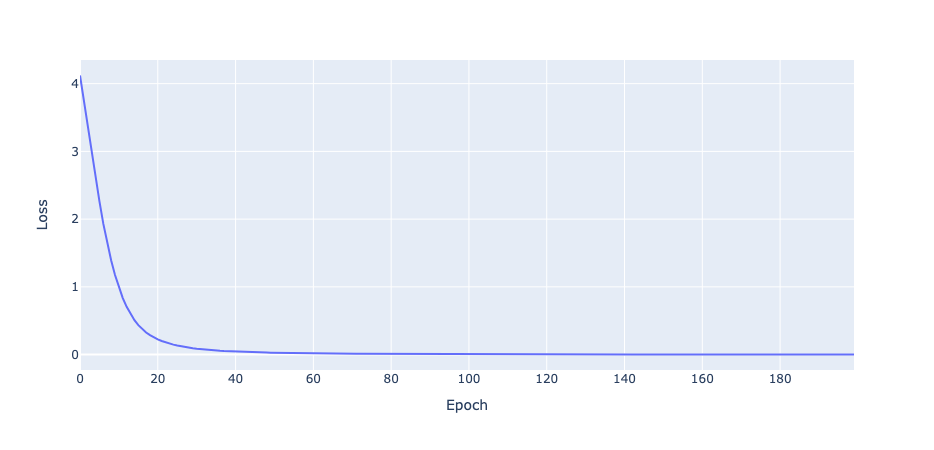
\includegraphics[scale=0.4]{fixed_length.png}

    \textbf{Figure 1: Loss Training on 200 Epochs}
\end{center}


I was surprised to find that even though the problem is simple, it wasn't able to achieve 100$\%$ accuracy on the validation set, but rather plateaus at around 96$\%$ for $n = 2, 3$. I printed out some of the incorrect predictions and found that the incorrect predictions are usually because the numbers are very close. Here are some examples:

\begin{center}
    \begin{tabular}{c c c}
        Input & Prediction & Actual \\
        $[53, 54]$ & 53 & 54 \\
        $[7, 6]$ & 6 & 7 \\
        $[49, 53]$ & 49 & 53 \\
        $[44, 45, 15]$ & 44 & 45 \\

    \end{tabular}
\end{center}

Although the model is generalizing, it still fails on some edge cases, which is interesting in terms of why that might be the case. This will be discussed further in the experiments section.

Furthermore, this model is only trained on fixed length lists and can only handle numbers up to the vocab size. This is a limitation because transformers have a fixed context length, which represents the cap on the input sequence, and a fixed vocab size, which represents the tokens that the transformer can recognize. 

\subsection{Variable Length Lists}

The next variation I did was training a model to take the max of variable length lists to get around the fixed length list limitation found in the previous section. This is similar to the previous experiment, but the data generation is different. Other than some duplicate code and code to generate graphs, all of this code was written by me in a file called ``variable$\_$length.ipynb."

In the fixed length data generation, we generated all possible combinations of a list of numbers of a fixed length based on the vocab size. For lists of size 2, there are $\text{D$\_$VOCAB}^2$ combinations, and so on. However, for variable length lists, generating all combinations would be too computationally expensive. 

Instead, we first choose a random length for the list from 1 to 10, then generate random numbers to fill the list, and fill the remaining unfilled spaces with 0 as filler. To separate the training and testing data, we hash the list that we train on and ensure that the same list is not generated in the testing data. This way, we can ensure that the model is generalizing and not memorizing the training data. Note that although this is a "variable length list" problem, the model still has a cap on the input sequence length since the context length is fixed for the transformer, so we can only generate variable length lists up to the context length. 

\subsubsection{Considerations and Limitations}
Although intuitively, this problem seems harder than finding the maximum of two numbers, the model was able to learn this task very quickly and achieve a much higher test accuracy of about 99.92$\%$. The loss plotted for 200 epochs is shown below:
\begin{center}
    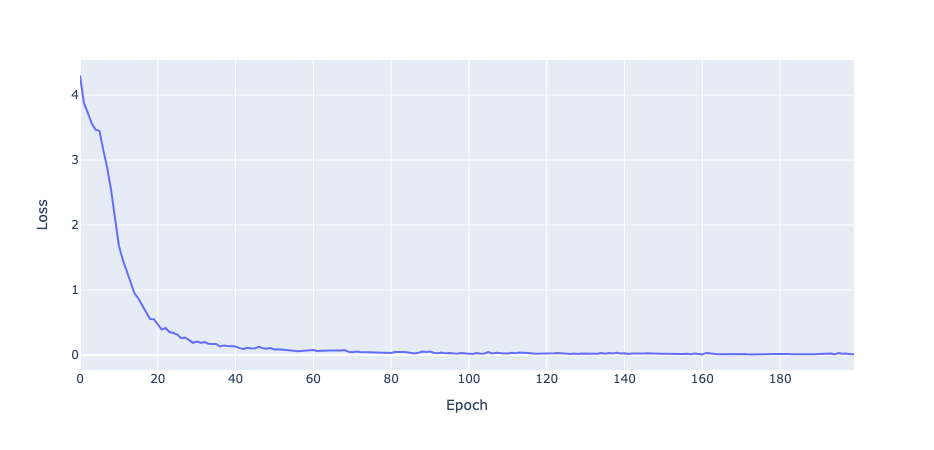
\includegraphics[scale=0.4]{variable_length.png}

    \textbf{Figure 2: Loss Training on 200 Epochs}
\end{center}

Compared to the graph for the fixed length lists, the loss of this graph is much less steady. It seems to have a consistent bump around epoch 10, which may be the model learning to generalize. However, this model does manage to achieve a higher validation accuracy than the fixed length model. This may be due to differences in data generation, where in this problem, the model actually sees all the numbers it has to distinguish rather than having a subset of numbers hidden away in the validation set. For example, the nature of the data generation in the previous iteration makes it so that the model never sees the combination of [44, 45] together. In this variation, although it might never see the exact sequence [44, 45, 0, 0, 0, 0, 0, 0, 0, 0], it might see something like [3, 44, 45, 0, 0, 0, 0, 0, 0, 0] and thus have an advantage. The hashing only ensures that the exact sequence of numbers is not in the testing set, so this would imply that the model can perform equally as well on the same numbers in different orders. 

The limitations of this model are similar to the fixed length model, where the model can only handle numbers up to the vocab size.


\subsection{Encoded Numbers}
Because of the consistent limitation of the vocab size, I wanted to see if the numbers could be encoded in a way such that the model could handle arbitrarily large numbers and predict the maximum of these numbers. I ended up spending a bulk of my time on this section of the project and found some interesting results. In this section, I will walk through the learning process of getting this to work, talk about how the numbers are encoded, the results of the training, and improvements I made on the encoding to get better results. All of the code that was written in these sections were written by me.

In the previous experiments, the list was not encoded at all, and the vocab size was a hard limit in what numbers that the transformer could recognize. If the vocab size was 64, then we could only compare numbers up to 63 (since we include 0). To get around this, I encoded the numbers in the list as their single digit values (This is similar to how GPT encodes words as partitions, like splitting ``bottle" into ``bot" ``tle"). For example, the number 123 would be encoded as $[1, 2, 3]$. This way, the model can recognize any number of any size up to a bound by the context length. Thus, an input token which represents comparing 231 and 39503 might look like this:
$$
[2, 3, 1, 11, 11, 10, 3, 9, 5, 0, 3]
$$
where 11 represents filler and 10 represents the split between the two numbers. 

Compared to the past two problems, predicting the maximum of these encoded numbers was much harder. I couldn't just predict the next number in the sequence as the maximum because the model's vocab size was too small (12 in this case). Thus, I had to predict a sequence of numbers instead that represents the largest number in the encoded format. I chose to predict the last sequence of five numbers in the list, which the model should predict as the maximum. A visualization of this is shown below:

\begin{center}
    $[2, 3, 1, 11, 11, 10, \text{\hl{3}}, \text{\hl{9}}, \text{\hl{5}}, \text{\hl{0}}, \text{\hl{3}}]$

    \textbf{The numbers highlighted in yellow are the indices the model should predict}
\end{center}

As it turns out, this doesn't make any sense because the model is not able to predict the maximum of the list if it didn't see the second half of the list, so the results were pretty random. It was a mistake on my part because I miscalculated that the model is not able to look ahead. This is a limitation of the transformer model, where the attention of the token is only based on the tokens before it.Even though this is an incorrect way to train the model, the results were still interesting and will be discussed in the experiments section. This code can be found under the file called ``encoding.ipynb''. 

\subsection{Improved Encodings}
After this initial failure, I experimented with different encodings, and eventually settled on the encoding as follows. The number 63 represents the start of the first number, the number 64 represents the start of the second number, and the number 65 represents the start of the answer. The numbers are then encoded as their single digit values, with leading zeroes added to make the length of the number 5. For example, the comparison of 783 and 28392 would be tokenized as
$$
[63, 0, 0, 7, 8, 3 64, 2, 8, 3, 9, 2, 65, \text{\hl{2}}, \text{\hl{8}}, \text{\hl{3}}, \text{\hl{9}}, \text{\hl{2}}]
$$

Some changes I made were changing the filler to appear at the front of the numbers. This way, the corresponding units places of the numbers are always at the same indices. Furthermore, I chose to use 63, 64, and 65 as markers instead of 10 so there is more separation in value between what numbers are important and what are just markers. 

To address the issue from the last encoding, I trained the model to predict the last five numbers in the list, at which point the model should have been able to see both the numbers. Note that when predicting the last five numbers, the model is not able to see the last five values which give away the answer. Thus, we know that the model is not just outputting the last five numbers, but is actually learning to take the maximum of the two numbers. This can be checked by switching the last five numbers to 0's, where the result is the same.

The numbers are generated by first generating two random numbers from the range of 0 to 99999, then encoding them as described above. The numbers are also hashed so that there is no overlap between the training and testing data.

\subsubsection{Considerations and Limitations}
I was surprised to see that the model did \textbf{not} learn this task very well despite the improvements in the encoding. There was essentially no difference in the accuracy of the improved encoding versus the original encoding. This can be best visualized by looking at the validation accuracy over time. 

\begin{center}
    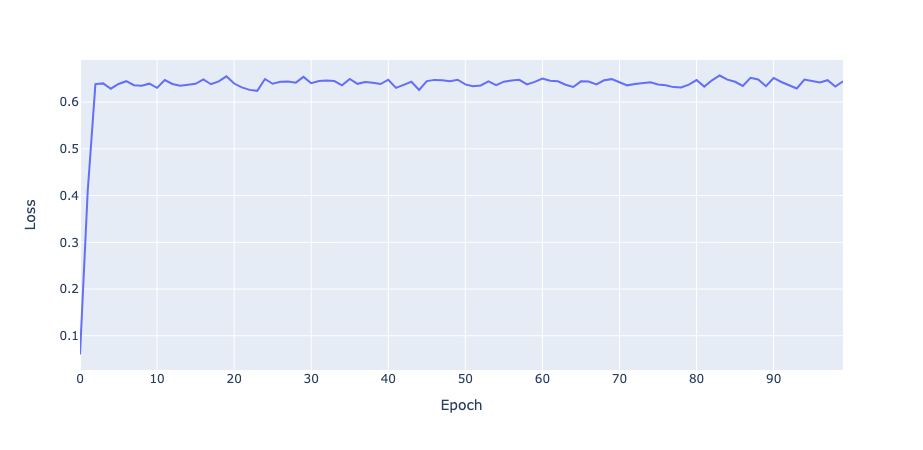
\includegraphics[scale=0.4]{encoding_answer.png}

    \textbf{Figure 3: Validation on 200 Epochs}

\end{center}

We see that in this graph, the accuracy plateaus at around 0.6 and wavers. Here are some of the inputs and predictions that the model made.

\begin{center}
    \begin{tabular} {c c c}
        Input & Prediction & Actual \\
        80828, 31326 & 81826 & 80828 \\
        72335, 26144 & 72144 & 72335 \\
        88101, 89268 & 88108 & 89268
    \end{tabular}
\end{center}

Based on these results, we see that the good thing is that it is not making up numbers, and it is taking the corresponding numbers in the right units place, just from the wrong number. It seems to be comparing the numbers in a certain way, but it is not able to remember which number it should keep taking from (the greater number) and rather makes a decision at each step. Based on this, I experimented with increasing the number of attention heads to 2 and increasing the number of layers to 2 so that the model has more expressive power. 

\begin{center}
    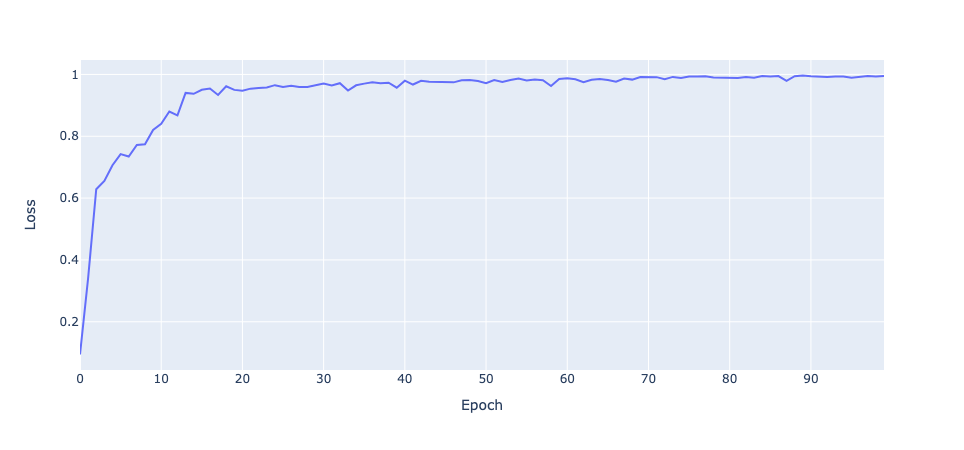
\includegraphics[scale=0.4]{encoding_more_heads.png}

    \textbf{Figure 4: Validation on 200 Epochs}
\end{center}

After increasing the attention heads and the number of layers, our validation accuracy is almost 100$\%$ after 200 epochs! This is a huge improvement from the previous model, and it seems that the model is able to learn the task when increasing the complexity of it. This probably stems from the fact that with two attention heads, it can keep track of the two numbers better, and two layers means that it can remember which number was greater and keep copying values from that number. 

\section{Attention Patterns}

Now that we have trained all the models to achieve high accuracy, we can look at the attention patterns of the models to gain insight into what is important to the model when taking the maximum. 

\subsection{Fixed Length Lists}

The attention patterns of the fixed length lists model are shown below.

\begin{center}
    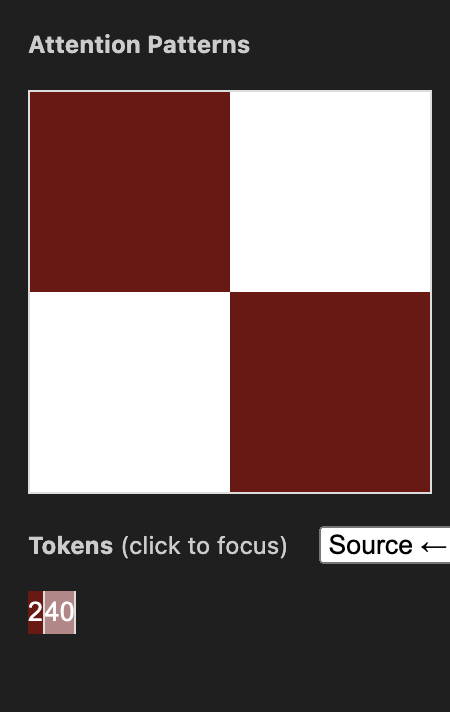
\includegraphics[scale=0.4]{att_fixed.png}
    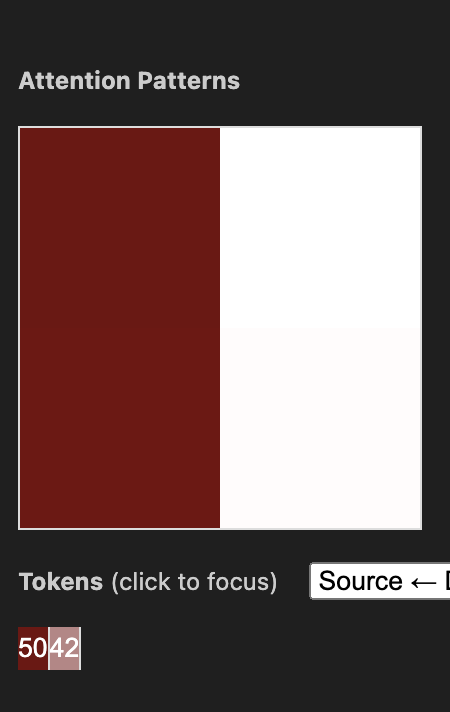
\includegraphics[scale=0.4]{att_fixed2.png}
    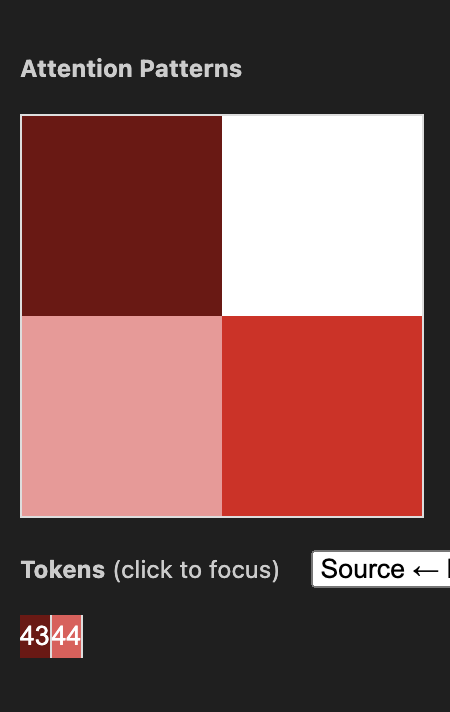
\includegraphics[scale=0.4]{att_fixed_edge.png}

    \textbf{Figure 5: Attention Patterns for Fixed Length Lists}
\end{center}

These images show the attention patterns for fixed lengths of size 2. Note that we only care about the patterns in the second row of each image, because the first token represented in the first row can only pay attention to itself. 

From the first two images, we see that generally, the second token pays attention to the token with the greater value. For example, with $[2, 40]$, the second token looks at itself because it is greater than 2, and with $[50, 42]$, the second token looks at the first token because it is greater. This is a good sign because this means that the model is paying attention to the right token when taking the maximum. 

The image on the right is an example of an attention pattern when the model fails to predict the maximum. In this case, the attention is accordingly confused and split across both tokens. This is a sign that the model is not memorizing the data, but rather split on which token to pay attention to, and this may be because the numbers are too close in value. The model may not have too much training on making decisions between numbers that are close in value, and thus fails in this case.

\subsection{Variable Length Lists}

\begin{center}
    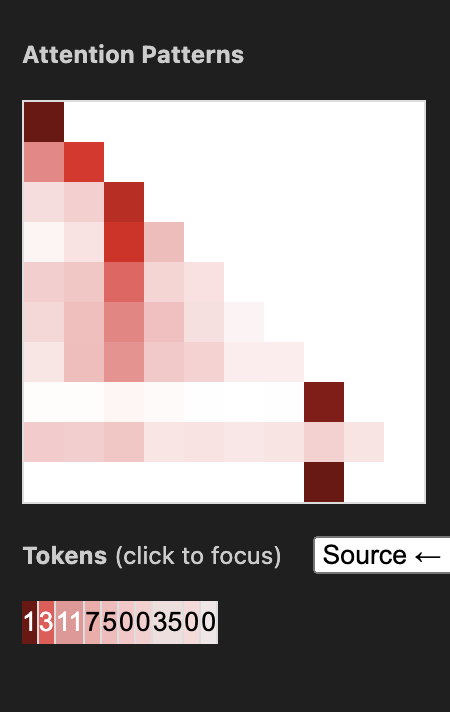
\includegraphics[scale=0.4]{images/att_variable.png}
    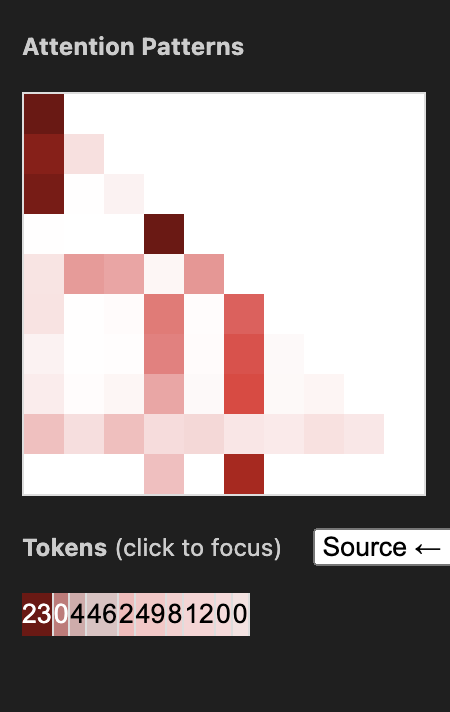
\includegraphics[scale=0.4]{images/att_variable2.png}
    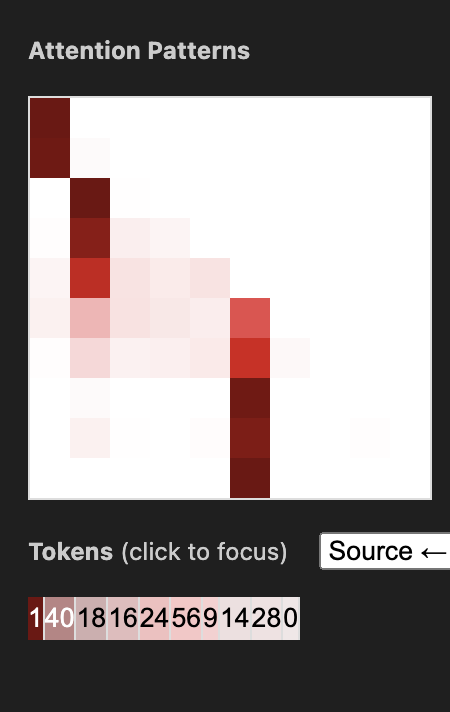
\includegraphics[scale=0.4]{images/att_variable3.png}

    \textbf{Figure 6: Attention Patterns for Variable Length Lists}
\end{center}

The attention patterns for the variable length lists model are shown above. These attention patterns are more involved than the last example. Unlike last time, we can look at the progression of attention as we increment through the list. 

We can make the observation that the model keeps track of the highest token so far as it increments through the list. This can be seen by the dark vertical lines that follow the highest token in the list and the white to the right of these vertical lines. This means that even though we increment and discover new numbers, the model still pays attention to the previous greatest element. At the last element, the model pays the most attention to the greatest element in the list because the attention of the last element signifies what the prediction will output. These attention patterns show that the model is learning to keep track of the greatest element throughout the list and copy it as the output.

\subsection{Encoded Numbers}
\begin{center}
    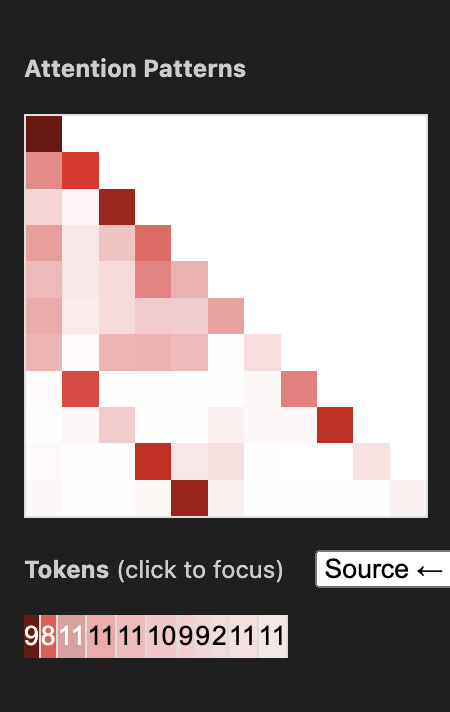
\includegraphics[scale=0.4]{images/att_encoding1.png}
    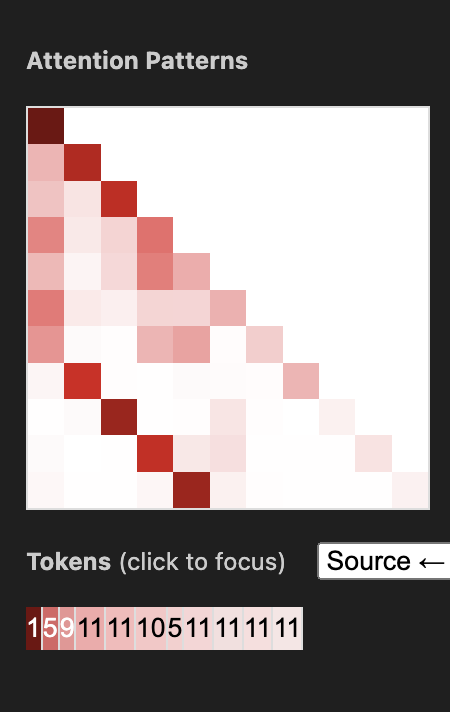
\includegraphics[scale=0.4]{images/att_encoding2.png}
    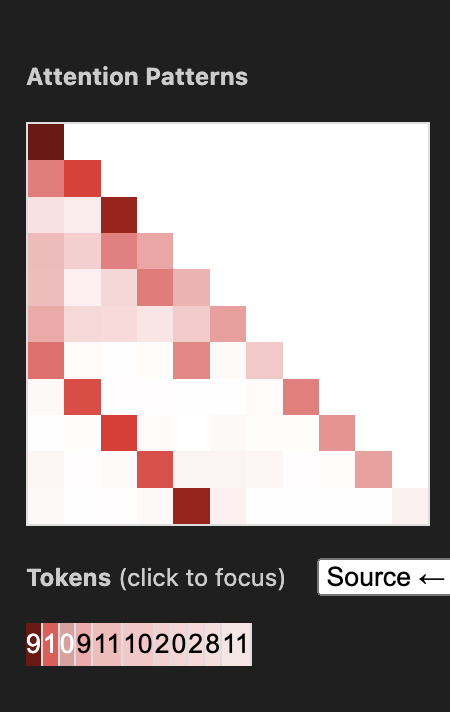
\includegraphics[scale=0.4]{images/att_encoding3.png}

    \textbf{Figure 7: Attention Patterns for Encoded Numbers}
\end{center}

The attention patterns for the naive encoding are shown above when there is one attention head and one layer. We see that for the last five attention patterns, they pay attention to the corresponding units place of the first number, seen by the two diagonals. This is a good sign because it means that the model is comparing the numbers in the right way. However, because the tokens are not set up in the right way, it's not actually able to compare it to the second number and thus fails. It is still interesting to see that it has the right idea in comparing the same units digits. 

\subsection{Improved Encodings}
\begin{center}
    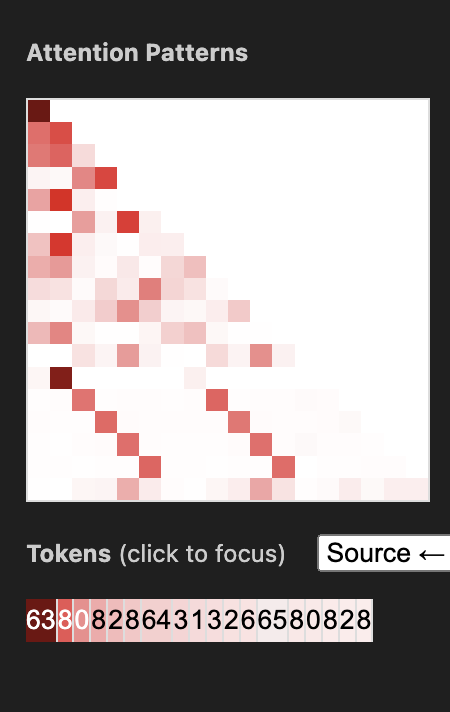
\includegraphics[scale=0.4]{images/att_encoding_1hd1.png}
    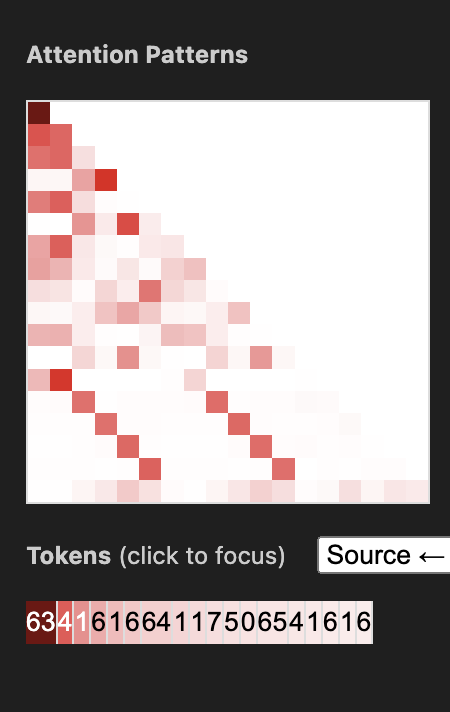
\includegraphics[scale=0.4]{images/att_encoding_1hd2.png}
    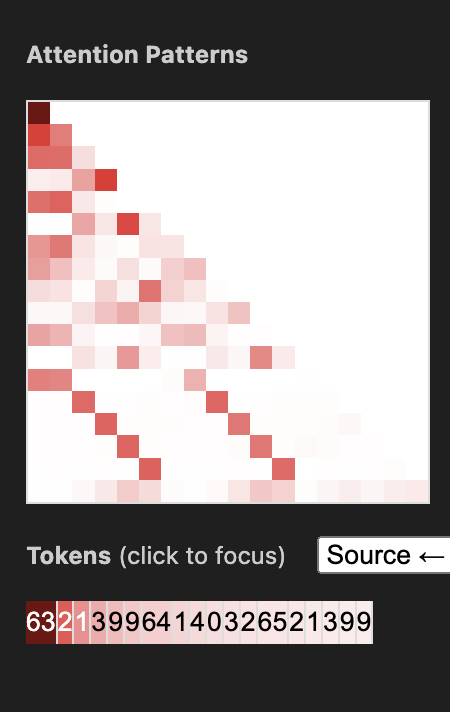
\includegraphics[scale=0.4]{images/att_encoding_1hd3.png}

    \textbf{Figure 8: Attention Patterns for Improved Encodings with 1 Head}
\end{center}

\begin{center}
    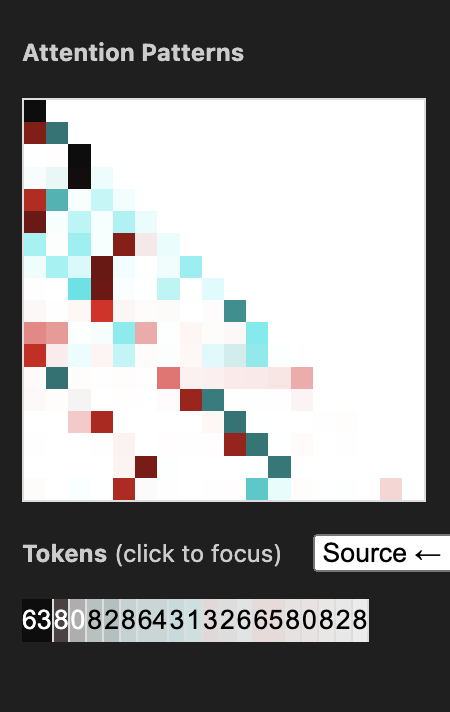
\includegraphics[scale=0.4]{images/att_encoding_2hd.png}
    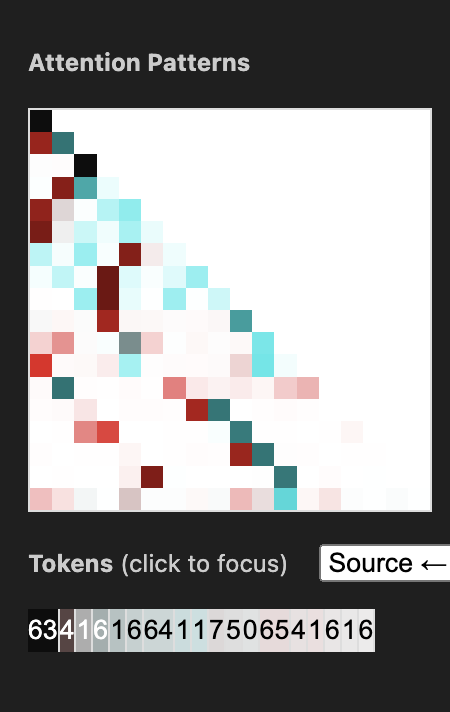
\includegraphics[scale=0.4]{images/att_encoding_2hd2.png}
    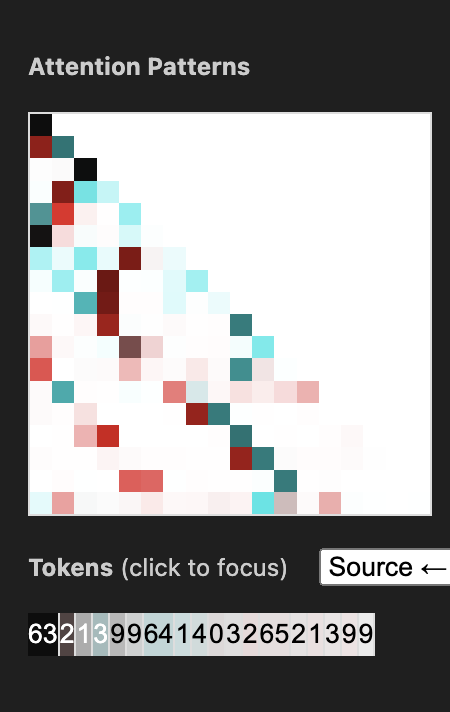
\includegraphics[scale=0.4]{images/att_encoding_2hd3.png}

    \textbf{Figure 9: Attention Patterns for Improved Encodings with 2 Heads}
\end{center}

The attention patterns for the improved encodings are shown above, where the top three images are for the model with one attention head and one layer, and the bottom three images are for the model with two attention heads and two layers.

For the single attention head attentions, we see that they are essentially doing the same thing as the naive encodings, where they are comparing the corresponding units place of the two numbers. However, it was stated before that the model probably is not able to remember which number it should be copying from, and thus the accuracy is not that high.

For the two attention head two layer attentions, we see that the attention is a little bit more random. Note that the blue cells represent one attention head and the red ones represent another. Upon closer inspection, we can see that the model either comparing the two corresponding units places of the two numbers, or it is comparing two digits next to each other in the same number. Because there are more attention heads now, the model is able to keep track of more numbers, and thus is able to remember which number it should be copying from. Looking at digits next to each other in the same number might serve as a way to remember what number it should be copying from.

\section{Conclusion} 

In this paper, we introduced a simple algorithmic problem, taking the maximum of numbers, and worked on training a transformer model to learn variations of this problem. This project has shown that there is a lot of interpretability that can be done on even a simple algorithmic problem. Although we didn't observe any grokking, it was interesting to work through the encodings and observe what the limitations of a single-head single-layer model might be and how changing that has an effect on the learning.

For future work, an analysis of the weights of each of the heads can be done to find specifics as to what the model is learning to further support our hypotheses. This framework can also be extended to different problems, such as sorting lists or an artificial algorithmic problem.

\newpage
\bibliographystyle{alpha}
\bibliography{sample}

\end{document}